\documentclass[%
	paper=a4,%
	twoside=true,%
	draft=false,%
	abstract=false]{scrartcl}

\usepackage[utf8]{inputenc}
\usepackage[english]{babel}
\usepackage{microtype}
\usepackage{graphicx}
\usepackage[load-configurations=binary]{siunitx}
	\DeclareSIUnit\Molar{\textsc{m}}
\usepackage{svn-multi}
\usepackage{subfig}
\usepackage{booktabs}
\usepackage{fancyhdr}
\usepackage{tikz}
\usepackage{pgfplots}
\usepackage[numbers,square,sort&compress]{natbib}
\usepackage{scrtime}
\usepackage[version=3]{mhchem}
\usepackage{setspace}
	%\doublespacing
	%\onehalfspacing
\usepackage{lineno}
	\linenumbers\modulolinenumbers[2]
\usepackage{lastpage}	
\usepackage{todonotes}
\usepackage{xspace}
\usepackage[autostyle]{csquotes}
\usepackage[backref]{hyperref}
 
% Subversion Information
\svnidlong
{$HeadURL$}
{$LastChangedDate$}
{$LastChangedRevision$}
{$LastChangedBy$}
\svnid{$Id$} 
 
\pagestyle{fancy}
\fancyfoot{}
\fancyfoot[OR]{\tiny Typeset on \today\ at \thistime\ from \href{\svnkw{HeadURL}}{Revision \svnkw{LastChangedRevision}}, committed on \svnkw{LastChangedDate} | Page \thepage\ of \pageref{LastPage}}
\fancyfoot[EL]{\tiny Page \thepage\ of \pageref{LastPage} | Typeset on \today\ at \thistime\ from \href{\svnkw{HeadURL}}{Revision \svnkw{LastChangedRevision}}, committed on \svnkw{LastChangedDate}}
 
\newcommand{\imsize}{\linewidth}

\newcommand{\footremember}[2]{\footnote{#2}\newcounter{#1}\setcounter{#1}{\value{footnote}}}
\newcommand{\footrecall}[1]{\footnotemark[\value{#1}]}

\newcommand{\superscript}[1]{\ensuremath{^{\textrm{#1}}}}
\newcommand{\subscript}[1]{\ensuremath{_{\textrm{#1}}}}

\newcommand{\ie}{i.\,e.}
\newcommand{\Ie}{I.\,e.}
\newcommand{\eg}{e.\,g.}
\newcommand{\Eg}{E.\,g.}
\newcommand{\twod}{2\textsc{d}\xspace}
\newcommand{\threed}{3\textsc{d}\xspace}
 
\title{Acinar growth over lung development}
\subtitle{Revision \svnkw{LastChangedRevision} | Typeset on \today\ at \thistime}

\author{%
	David Haberthür\footremember{ana}{Institute of Anatomy, University of Bern, Switzerland}%
	\and Marco Stampanoni\footremember{psi}{Swiss Light Source, Paul Scherrer Institut, Villigen, Switzerland}\footremember{eth}{Institute for Biomedical Engineering, Swiss Federal Institute of Technology and University of Zürich, Switzerland}%
	\and Johannes C. Schittny\footrecall{ana}%
	}
\date{}

\begin{document}
\maketitle

\begin{abstract}
Here be the Abstract\ldots
\end{abstract}

\section{Introduction}\label{sec:Introduction}
The pulmonary acinus (the gas-exchange volume in the lung which is ventilated by one purely conducting airway~\cite{Rodriguez1987}) represents the functional unit of the lung parenchyma. Due a restricted availability of high resolution three-dimensional imaging methods the knowledge about the development of the pulmonary acini is limited. Using synchrotron radiation based tomographic microscopy \cite{Haberthuer2010a} we developed a method to evaluate the volume of single acini throughout postnatal lung development\todo{Why did we want to do that? Do we need to list/explain existing prior models?}. In pre-experiments assessing the lung structure using three-dimensiona visualizations of synchrotron radiation based tomographic microscopy datasets we have seen that the functinal lung units---the so-called acini---seen to grow to a larger extent than expected from \emph{simple} lung development.

The lung structure can be assessed using using stereology~\cite{Hsia2010}, as shown by \citet{Tschanz2002}. Such an analysis is generally based on serial sections of the sample, thus the extracted information is a two-dimensional description \blockquote[\cite{Tschanz2002}]{of the parenchymal air space geometry and, due to geometric laws, it is not allowed to extrapolate these \twod statements directly to \threed structures}. With stereological methods it is farily easy to extract global volume information \todo{From a region, from a ROI?}, but it not easily possible to extract such information from a functional unit of any organ, since it cannot easily be judged which detail on the microscopy slide belong to which functional unit in the three-dimensional compound.


\begin{itemize}
	\item Classic SRXTM
	\item WF-SRXTM~\cite{Haberthuer2010}
\end{itemize}

\section{Materials \& Methods}\label{sec:MM}
\subsection{Rat lung samples}
Rat lung samples, prepared according to \cite{Tschanz2002,Luyet2002} were used as test objects. Briefly, lungs of Sprague-Dawley rats were filled with \SI{2.5}{\percent} glutaraldehyde (\cf{CH2(CH2CHO)2}) in \SI{0.03}{\Molar} potassium-phosphate buffer (pH 7.4) by instillation via tracheotomy at a constant pressure of \SI{20}{\centi\meter} water column. In order to prevent recoiling of the lung, this pressure was maintained during glutaraldehyde-fixation for a minimum of two hours. Subsequently, the lungs were dissected free and immersed in toto in the same fixative at a temperature of \SI{4}{\celsius} for at least \SI{24}{\hour}.

The samples were postfixed with \SI{1}{\percent} osmium tetroxide (\cf{OsO4}) and stained with \SI{4}{\percent} uranyl nitrate (\cf{UO2(NO3)2}) to increase the x-ray absorption contrast, dehydrated in a graded series of ethanol and embedded in paraffin using Histoclear (Merck KGaA, Darmstadt, Germany) as an intermedium. The lung samples were mounted onto standard scanning electron microscopy sample holders (PLANO GmbH, Wetzlar, Germany) using paraffin~\cite{Tsuda2008}.

The handling of animals before and during the experiments, as well as the experiments themselves, were approved and supervised by the Swiss Agency for the Environment, Forests and Landscape and the Veterinary Service of the Canton of Bern, Switzerland.

\subsection{Tomographic data acquisition}
The experiments were performed at the TOMCAT beamline at the Swiss Light Source, Paul Scherrer Institut, Villigen, Switzerland~\cite{Stampanoni2006a}. The samples were scanned at \SI{12.6}{\kilo\electronvolt}. After penetration through the sample, the x-rays were converted into visible light by a YAG:Ce scintillator (\SI{18}{\micro\meter} thickness, Crismatec Saint-Gobain, Nemours, France). Projections were magnified by diffraction limited microscope optics (10\(\times\) magnification) and digitized by a high-resolution 2048\(\times\)2048 pixel CCD camera (pco.2000, PCO AG, Kelheim, Germany) with \SI{14}{\bit} dynamic range. The detector was operated in 2\(\times\)2 binning mode. As a result, the pixel size was \SI{1.48}{\micro\meter} and the exposure time was \SI{175}{\milli\second}\todo{already mention Wide-Field Scanning here?}.

To study the alveolar septa, a resolution in the order of one micron is required. Since we selectively wanted to choose an alveolus/multiple alveoli, a large sample volume had to be scanned. Usually, a large field of view resulting in a large sample volume can only be acquired with low magnification and vice-versa. Thus, the full volume of our samples would not have fit inside the field of view of the TOMCAT beamline at the chosen optical properties (\(1.52\times1.52\times\)\SI{1.52}{\milli\meter}).

To enhance the field of view of the TOMCAT beamline at the chosen optical configuration, we obtained tomographic datasets using a so called wide field scan~\cite{Haberthuer2010}. Briefly, several partial scans with an optimized amount of projections spanning an enlarged field of view have been independently acquired. Prior to reconstructing the tomographic dataset, these projections have been merged to one large projection spanning the desired field of view. With this approach we increased the available field of view at TOMCAT three-fold, while keeping the voxel size and reconstruction quality on the desired level and avoiding the aforementioned trade-off between voxel size and sample volume.

\subsection{Visualization and Extraction of Acini}
The tomographic datasets of the sample three-dimensionally analyzed and visualized using MeVisLab (Version 2.1 (2010-07-26 Release), MeVis Medical Solutions AG and Fraunhofer MEVIS - Institute for Medical Image Computing, Bremen, Germany). The tomograhic dateset was loaded, processed and visualized\todo{Write exact details of processing network}. Airway segments were extracted using a threshold interval based region growing algorithm~\cite{Zucker1976}. A seed point for the region growing algorithm was manually defined inside the terminal broncioloe/alveolar duct on one of the most proximal slices. The segmented airways have been visualized and cropped to a promising region of interest and exported as DICOM-file to facilitate further processing using ImageJ~\cite{Abramoff2004} and the Stepanizer~\cite{Tschanz2010}.

\begin{itemize}
	\item Extraction of Acinus
	\item Manhole Covers
	\begin{itemize}
		\item Morphological Criteria $\rightarrow$ Detection of ``Entrance Point'' into Acinus
		\item Threshold based, seeded Region Growing
		\item Pixel Volume counting
	\end{itemize}
	\item Data to measure:
	\begin{itemize}
		\item Acinar volume
		\item Acinar surface
		\item Number of alveoli
		\item Mean alveolar volume
		\item Total alveolar volume
		\item Total ductal volume
	\end{itemize}
\end{itemize}

\section{Results}\label{sec:Results}
For each day and sample we extracted multiple\todo{how many exactly?} acini with the \emph{Manhole Cover}-method.

The data has been analyzed using R (Version 2.12.1 (2010-12-16)~\cite{R}. A summary of the extracted acinar volumes is shown in \autoref{tab:summary}

% FROM R
%summary(Data)
%       D4                D10                 D21                 D36                D60           
% Min.   :2.32e-05   Min.   : 0.000510   Min.   : 0.000858   Min.   : 0.00608   Min.   :3.320e-06  
% 1st Qu.:9.15e-04   1st Qu.: 0.004510   1st Qu.: 0.010095   1st Qu.: 0.03130   1st Qu.:2.615e-02  
% Median :2.14e-03 & 0.007520   Median : 0.021600   Median : 0.04830   Median :5.370e-02  
% Mean   :3.64e-03   Mean   : 0.009208   Mean   : 0.030228   Mean   : 0.05526   Mean   :6.227e-02  
% 3rd Qu.:6.07e-03   3rd Qu.: 0.012800   3rd Qu.: 0.045300   3rd Qu.: 0.07630   3rd Qu.:8.480e-02  
% Max.   :1.35e-02 & 0.025200 & 0.098600 & 0.13900 &1.740e-01  
% NA's   :3.30e+01   NA's   :37.000000   NA's   :51.000000   NA's   :41.00000   NA's   :5.200e+01  
\begin{table}
	\centering
	\caption{Summary of the extracted Data. All volumes are givenin \si{\micro\litre}}
	\begin{tabular}{rccccc}
		\toprule
		& Day 04 & Day 10 & Day 21 & Day 36 & Day 60\\
		\midrule
		Minimum 						& \num{2.32e-05} & \num{0.000510} & \num{0.000858} & \num{0.00608} & \num{3.320e-06}\\
		1\superscript{st} Quantile 	& \num{9.15e-04} & \num{0.004510} & \num{0.010095} & \num{0.03130} & \num{2.615e-02}\\
		Median 							& \num{2.14e-03} & \num{0.007520} & \num{0.021600} & \num{0.04830} & \num{5.370e-02}\\
		Mean 							& \num{3.64e-03} & \num{0.009208} & \num{0.030228} & \num{0.05526} & \num{6.227e-02}\\
		3\superscript{rd} Quantile 	& \num{6.07e-03} & \num{0.012800} & \num{0.045300} & \num{0.07630} & \num{8.480e-02}\\
		Maximum 						& \num{1.35e-02} & \num{0.025200} & \num{0.098600} & \num{0.13900} & \num{1.740e-01}\\
		\bottomrule
	\end{tabular}
	\label{tab:summary}
\end{table}


\begin{figure}
	\centering
	%% Created by tikzDevice version 0.5.3 on 2011-02-17 11:33:02
%\documentclass{article}
%\usepackage{tikz}
%
%\usepackage[active,tightpage]{preview}
%
%\PreviewEnvironment{pgfpicture}
%
%\begin{document}
%%%%%%%%%%%%%%%%%%%%%%%%%%%%%%%%%%%%%%%%%
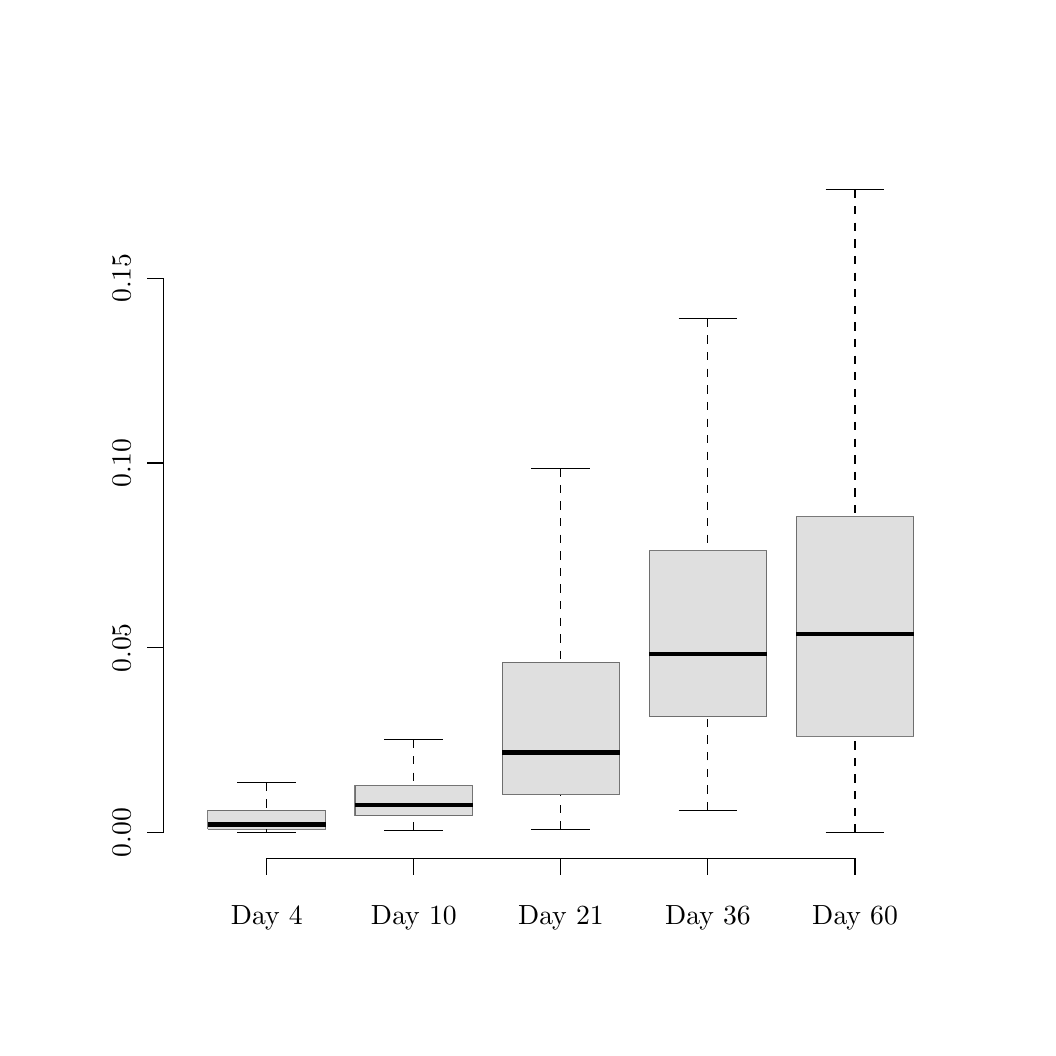
\begin{tikzpicture}[x=1,y=1]
\begin{scope}
%%%%%%%%%%%%%%%%%%%%%D04
\draw[dashed] ( 86.40, 70.52) -- ( 86.40, 71.71);
\draw[dashed] ( 86.40, 88.52) -- ( 86.40, 78.60);
\draw[] ( 75.77, 70.52) -- ( 97.02, 70.52);
\draw[] ( 75.77, 88.52) -- ( 97.02, 88.52);
\draw[fill=lightgray,semitransparent] ( 65.14, 71.71) --
	(107.65, 71.71) --
	(107.65, 78.60) --
	( 65.14, 78.60) --
	( 65.14, 71.71);
\draw[ultra thick] ( 65.14, 73.35) -- (107.65, 73.35);	
%%%%%%%%%%%%%%%%%%%%%D10
\draw[dashed] (139.54, 71.17) -- (139.54, 76.51);
\draw[dashed] (139.54,104.14) -- (139.54, 87.58);
\draw[] (128.91, 71.17) -- (150.16, 71.17);
\draw[] (128.91,104.14) -- (150.16,104.14);
\draw[fill=lightgray,semitransparent] (118.28, 76.51) --
	(160.79, 76.51) --
	(160.79, 87.58) --
	(118.28, 87.58) --
	(118.28, 76.51);
\draw[ultra thick] (118.28, 80.53) -- (160.79, 80.53);
%%%%%%%%%%%%%%%%%%%%%D21
\draw[dashed] (192.67, 71.64) -- (192.67, 84.24);
\draw[dashed] (192.67,202.16) -- (192.67,132.05);
\draw[] (182.05, 71.64) -- (203.30, 71.64);
\draw[] (182.05,202.16) -- (203.30,202.16);
\draw[fill=lightgray,semitransparent] (171.42, 84.24) --
	(213.93, 84.24) --
	(213.93,132.05) --
	(171.42,132.05) --
	(171.42, 84.24);
\draw[ultra thick] (171.42, 99.47) -- (213.93, 99.47);
%%%%%%%%%%%%%%%%%%%%%D36
\draw[dashed] (245.81, 78.61) -- (245.81,112.29);
\draw[dashed] (245.81,256.12) -- (245.81,172.38);
\draw[] (235.19, 78.61) -- (256.44, 78.61);
\draw[] (235.19,256.12) -- (256.44,256.12);
\draw[fill=lightgray,semitransparent] (224.56,112.29) --
	(267.07,112.29) --
	(267.07,172.38) --
	(224.56,172.38) --
	(224.56,112.29);
\draw[ultra thick] (224.56,134.99) -- (267.07,134.99);
%%%%%%%%%%%%%%%%%%%%%D60
\draw[dashed] (298.95, 70.49) -- (298.95,105.34);
\draw[dashed] (298.95,302.86) -- (298.95,184.67);
\draw[] (288.32, 70.49) -- (309.58, 70.49);
\draw[] (288.32,302.86) -- (309.58,302.86);
\draw[fill=lightgray,semitransparent] (277.70,105.34) --
	(320.21,105.34) --
	(320.21,184.67) --
	(277.70,184.67) --
	(277.70,105.34);
\draw[ultra thick] (277.70,142.20) -- (320.21,142.20);	
\end{scope}
\begin{scope}
\path[clip] (  0.00,  0.00) rectangle (361.35,361.35);

\draw[] ( 86.40, 61.20) -- (298.95, 61.20);
\draw[] ( 86.40, 61.20) -- ( 86.40, 55.20);
\draw[] (139.54, 61.20) -- (139.54, 55.20);
\draw[] (192.67, 61.20) -- (192.67, 55.20);
\draw[] (245.81, 61.20) -- (245.81, 55.20);
\draw[] (298.95, 61.20) -- (298.95, 55.20);

\node[anchor=base,] at ( 86.40, 37.20) {Day 4};
\node[anchor=base,] at (139.54, 37.20) {Day 10};
\node[anchor=base,] at (192.67, 37.20) {Day 21};
\node[anchor=base,] at (245.81, 37.20) {Day 36};
\node[anchor=base,] at (298.95, 37.20) {Day 60};

\draw[] ( 49.20, 70.49) -- ( 49.20,270.81);
\draw[] ( 49.20, 70.49) -- ( 43.20, 70.49);
\draw[] ( 49.20,137.26) -- ( 43.20,137.26);
\draw[] ( 49.20,204.03) -- ( 43.20,204.03);
\draw[] ( 49.20,270.81) -- ( 43.20,270.81);

\node[rotate= 90.00,anchor=base,] at ( 37.20, 70.49) {0.00};
\node[rotate= 90.00,anchor=base,] at ( 37.20,137.26) {0.05};
\node[rotate= 90.00,anchor=base,] at ( 37.20,204.03) {0.10};
\node[rotate= 90.00,anchor=base,] at ( 37.20,270.81) {0.15};

%\draw[] ( 49.20, 61.20) --
%	(336.15, 61.20) --
%	(336.15,312.15) --
%	( 49.20,312.15) --
%	( 49.20, 61.20);
\end{scope}
\end{tikzpicture}
%%%%%%%%%%%%%%%%%%%%%%%%%%%%%%%%%%%%%%%%%
%\end{document}
	\caption{BoxPlot of Data with removed outliers}
	\label{fig:boxplot}
\end{figure}

\begin{figure}
	\centering
	\pgfplotsset{width=.5\linewidth}
	\subfloat[Mean acinar volumes]{% !TEX root = ../acinus.tex

% \documentclass{article}
% \usepackage{tikz,pgfplots}
% \usepackage{siunitx}
% \usepackage[graphics,tightpage,active]{preview}
% \PreviewEnvironment{tikzpicture}
% \newcommand{\imsize}{\linewidth}
% \newlength\imagewidth           % needed for scalebars
% \newlength\imagescale           % ditto
% \begin{document}%
%%%%%%%%%%%%%%%%%%%%%%%%%%%%%%%%%%%%%%%%
	\begin{tikzpicture}
		\begin{axis}[%
			legend pos=south east,%
			scale only axis,%
			%ultra thick,%
			xlabel={Days},%
			ylabel={Volume [\si{\micro\litre}]},%
			xlabel near ticks,%
			ylabel near ticks,%
			xtick = data,%
			ytick = {0,0.02,...,0.11},%
			%ymajorgrids=true%
			]
			\addplot [blue,%
				mark=*,%
				semitransparent,%
				error bars/.cd,y dir=both,y explicit]
				coordinates {
 					(4,0.002595) +- (0.000308,0.000308)
					(10,0.012600) +- (0.001271,0.001271)
					(21,0.05602) +- (0.005973,0.005973)
					(36,0.084727) +- (0.006036,0.006036)
					(60,0.086460) +- (0.007447,0.007447)};
			\legend{Acini}
		\end{axis}
		\end{tikzpicture}
%%%%%%%%%%%%%%%%%%%%%%%%%%%%%%%%%%%%%%%%
% \end{document}
%Day	average	standard deviation	standard error of mean
%4	0.305	0.035	0.015
%10	0.508	0.048	0.022
%21	1.048	0.092	0.041
%36	2.062	0.141	0.063
%60	2.964	0.194	0.087}\\%
	\subfloat[Mean right lower lung lobe (RLL) volumes]{% !TEX root = ../acinus.tex

% \documentclass{article}
% \usepackage{tikz,pgfplots}
% \usepackage{siunitx}
% \usepackage[graphics,tightpage,active]{preview}
% \PreviewEnvironment{tikzpicture}
% \newcommand{\imsize}{\linewidth}
% \newlength\imagewidth           % needed for scalebars
% \newlength\imagescale           % ditto
% \begin{document}%
%%%%%%%%%%%%%%%%%%%%%%%%%%%%%%%%%%%%%%%%
	\begin{tikzpicture}
		%\tikzset{every mark/.append style={scale=4}}
		%\pgfplotsset{every axis legend/.append style={at={(0.8,0.08)},anchor=base}}
		\begin{axis}[%
			legend pos=south east,%
			scale only axis,%		
			%ultra thick,%
			xlabel={Days},%
			ylabel={Volume [\si{\centi\meter\cubed}]},%
			xlabel near ticks,%
			ylabel near ticks,%
			xtick = data,%
			%ytick = {0,5,...,35},%
			%ymajorgrids=true%
			]
			\addplot [red,%
				mark=square*,%
				semitransparent,%
				error bars/.cd,y dir=both,y explicit]
				coordinates {
 					(4,0.305) +- (0.015,0.015)
					(10,0.508) +- (0.022,0.022)
					(21,1.048) +- (0.041,0.041)
					(36,2.062) +- (0.063,0.063)
					(60,2.964) +- (0.087,0.087)};
		\legend{RLL}
		\end{axis}
		\end{tikzpicture}
%%%%%%%%%%%%%%%%%%%%%%%%%%%%%%%%%%%%%%%%
% \end{document}
%Day	average	standard deviation	standard error of mean
%4	0.305	0.035	0.015
%10	0.508	0.048	0.022
%21	1.048	0.092	0.041
%36	2.062	0.141	0.063
%60	2.964	0.194	0.087}\\%
	\subfloat[Volume increase based on day 4]{% !TEX root = ../acinus.tex

% \documentclass{article}
% \usepackage{tikz,pgfplots}
% \usepackage{siunitx}
% \usepackage[graphics,tightpage,active]{preview}
% \PreviewEnvironment{tikzpicture}
% \newcommand{\imsize}{\linewidth}
% \newlength\imagewidth           % needed for scalebars
% \newlength\imagescale           % ditto
% \begin{document}%
%%%%%%%%%%%%%%%%%%%%%%%%%%%%%%%%%%%%%%%%
	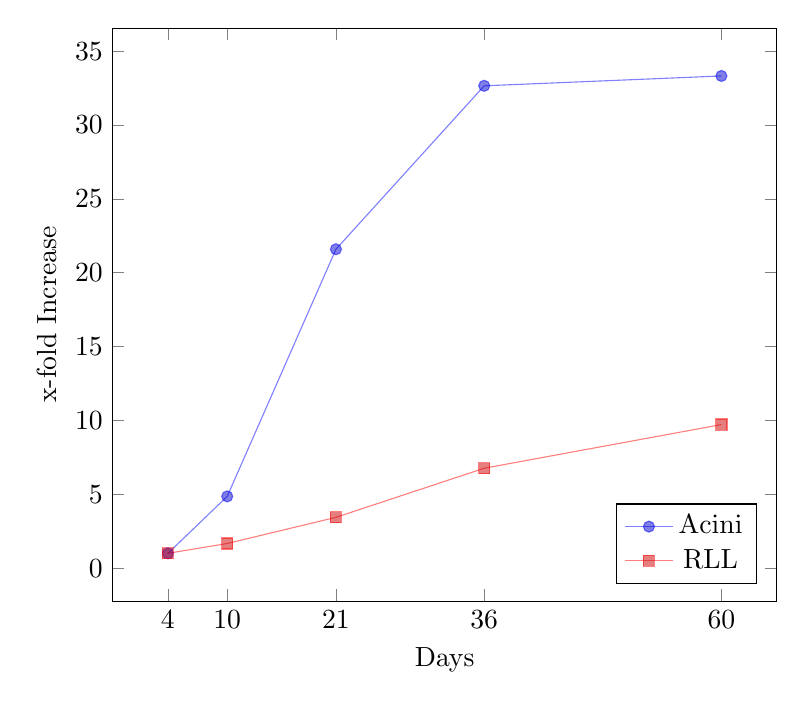
\begin{tikzpicture}
		\begin{axis}[%
			legend pos=south east,%
			scale only axis,%		
			%ultra thick,%
			xlabel={Days},%
			ylabel={x-fold Increase},%
			xlabel near ticks,%
			ylabel near ticks,%
			xtick = data,%
			ytick = {0,5,...,35},%
			%ymajorgrids=true%
			]
		\addplot+[semitransparent]
			coordinates{
		 		(4,1)
				(10,4.85549)
				(21,21.58767)
				(36,32.65010)
				(60,33.31792)
		};
		\label{plot:acini}
		\addplot+[semitransparent]
			coordinates{
				(4,1)
				(10,1.666)
				(21,3.436)
				(36,6.761)
				(60,9.718)
		};
		\label{plot:rul}
		\legend{Acini,RLL}
		\end{axis}
		\end{tikzpicture}
%%%%%%%%%%%%%%%%%%%%%%%%%%%%%%%%%%%%%%%%
% \end{document}}%
	\caption{Plot of increase in Volume for both Acini (\ref{plot:acini}) and right lower lung lobe (RLL, \ref{plot:rul}). While the volume of the right lower lung lobe increases approximately 10-fold over the first 2 months after birth, we see an approximately 33-fold increase in mean volume for the extracted acini from day \numrange{4}{60}.}
	\label{plot}
\end{figure}

We observed an approximately thirty-three-fold increase of the mean acinar volume during the postnatal lung development from days \numrange{4}{60} (33.25-fold, from \SIrange{0.00260}{0.08646}{\micro\litre}). During the same period the volume of the right lower lung lobe increases only approximately ten-fold (9.72-fold, from \SIrange{0.305}{2.964}{\centi\metre\cubed}, see \cite{Tschanz2003}), which results in an acinar growth 3.4 times larger than the right lower lung lobe volume.

\section{Discussion}\label{sec:Discussion}
We hypothesize that this large increase of the acinar volume can only be achieved by a conversion of the \numrange{2}{4} most distal purely conducting airways into alveolar ducts between birth and adulthood. As a consequence \numrange{4}{16} small acini have to be merged to a larger one. We expect that the increased complexity of the adult acini influences both ventilation and particle deposition.

\section{Acknowledgments}
\begin{itemize}
	\item Xris, Fede, Bernd
	\item Mohammed
	\item Sebastien? Or is he also on the author list?
	\item SNF
\end{itemize}
\bibliographystyle{unsrtnat}
\bibliography{../references}
 
\end{document}